%TrackingFilter.tex
\section{A Robust Tracking Filter for Bearings Measurements}\label{sec:TrackingFilter}
In this section, we detail the design and performance of a target tracking filter that uses bearings measurements. The Kalman-like hybrid nonlinear filter is stable and robust to synchronization error on the network and asynchronous transmissions of bearings data to the central processor (or any processor). The filter does not need very much more computation than a Kalman filter. We make the following assumptions upon the sensor network:

\begin{assumption}
Sensors are laid out randomly on the terrain--in particular, their coordinates follow a 2D Gaussian distribution.
\end{assumption}
\begin{assumption}
Each sensor's location is known through GPS or prior localization.
\end{assumption}
\begin{assumption}
The sensors are omnidirectional, i.e., they have a $360^\circ$ field of view.
\end{assumption}

To model general motion of an object on the plane, we use a constant acceleration point mass model for both the $x$ and $y$ coordinates of the object. This permits tracking both the motion of vehicles and human beings or animals with the same filter.
\begin{eqnarray}
% \nonumber to remove numbering (before each equation)
  \dot{\mathbf{x}} &=&\mathbf{v} \nonumber \\
  \dot{\mathbf{v}} &=& {\mathbf{a}}\nonumber \\
  \dot{\mathbf{a}} &=& \mathbf{\nu }_{2 \times 1}\nonumber\\
  \mathbf{x}&=&\left(\begin{array}{c} x \\y\end{array}\right),\quad   \mathbf{v}=\left(\begin{array}{c} v_x \\v_y\end{array}\right),\quad  \mathbf{a}=\left(\begin{array}{c} a_x \\a_y\end{array}\right)\nonumber\\
  {\nu }_{2 \times 1}&=&\left(\begin{array}{c} \nu_x \\\nu_y\end{array}\right),\quad
  \nu_x\sim N(0,\sigma_x), \nu_y\sim N(0,\sigma_y)\label{eqn:pointmassmodelcontinuous}
\end{eqnarray}
We rewrite the model in discrete time taking the sampling time $T$ of the sensors into account, stacking up the $x$ and $y$ dynamics on top of each other. From this point, boldface $\mathbf{x}$ will denote the overall state of the tracked object--$\left( x v_x a_x y v_y a_y\right)^T$.
\begin{eqnarray}
\mathbf{x}(k+1)&=&\mathbf{A}\mathbf{x}(k)+\mathbf{\nu}(k)\label{eqn:pointmassmodeldiscrete}\\
\mathbf{A}&=&\begin{pmatrix}
             \mathbf{A}_1 & \mathbf{0} \\
             \mathbf{0} & \mathbf{A}_1 \\
           \end{pmatrix}\nonumber\\
\mathbf{A}_1&=&\begin{pmatrix}
                 1 & T & {T^2\over 2} \\
                 0 & 1 & T \\
                 0 & 0 & 1 \\
               \end{pmatrix}\nonumber\\
\end{eqnarray}


\subsection{Constructing a Measurement}
The sensors output bearing to the tracked object which is also equivalent to measuring the slope $m_i(\mathbf{x}(k))={y(k)-y_i \over x(k)-x_i}$ of a line joining the sensor location $(x_i,y_i)$ to the tracked object at the sensing instant. We create a measurement function that consists in the  $y$-intercept of the line joining the sensor to the tracked object.
\begin{eqnarray}
z(k)&=&y_i-m_i(\mathbf{x}(k))x_i\nonumber\\
&=&y(k)-m_i(\mathbf{x}(k))x(k)=\mathbf{C}(\mathbf{x}(k))\mathbf{x}(k)\label{eqn:measurement},
\end{eqnarray}
where $\mathbf{C}(\mathbf{x}(k))=\left(-m_i(\mathbf{x}(k))\quad 0\quad 0\quad 1\quad 0\quad 0\right)$. Before we move to filter construction, we assume the slope measurement follows a normal distribution, which implies a normal distribution for the intercept when the sensor positions are known, which suggests a Kalman-filter structure.

\subsection{Kalman-like Nonlinear Hybrid Filter}
We construct our filter using the above measurement. We make assumptions standard in Kalman filtering: the initial condition of the moving object is a random variable uncorrelated to the state covariance $\mathbf{Q}$;  the measurement noise and state covariance are uncorrelated. The state covariance is a $6 \times 6$ matrix with only two non-zero elements $q_{33}=\sigma_x^2,\quad q_{66}=\sigma_y^2$. The measurement noise covariance has the form
\begin{equation}\label{eqn:Rk}
    \mathbf{R}_i(k)=x_i^2\mathbf{R},
\end{equation}
where $(x_i,y_i)$ is the location of the sensor that sends data at time $k$. If there is uncertainty in sensor positions, as when localization is being executed, the corresponding covariances can be added to the $\mathbf{R}_i(k)$. With all of these assumptions, the filter equations for the state estimate $\mathbf{\hat{x}}(k)$, the Kalman gain $\mathbf{K}(k)$, and the state covariance ${\Sigma}(k)$ can be written as:
 \begin{eqnarray}
 % \nonumber to remove numbering (before each equation)
   \mathbf{\hat{x}}(k+1) &=& \mathbf{A}\mathbf{\hat{x}}(k)+ \mathbf{K}(k)\left(y(k)-\mathbf{C}\left(\mathbf{x}(k)\right)\mathbf{\hat{x}}(k)\right)\label{eqn:Kalman-likeFilter}\\
   \mathbf{K}(k) &=& \left(\mathbf{A}{\Sigma}(k)\mathbf{C}\left(\mathbf{x}(k)\right)\right)\nonumber\\
   &&\times\left(\mathbf{C}\left(\mathbf{x}(k)\right){\Sigma}(k)\mathbf{C}\left(\mathbf{x}(k)\right)^T+\mathbf{R}_i(k)\right)^{-1} \label{eqn:FilterGainUpdate}\\
   {\Sigma}(k+1)&=& \mathbf{A}{\Sigma}(k)\mathbf{A}^T+\mathbf{Q}\nonumber\\
   &&-\mathbf{K}(k)\left(\mathbf{C}\left(\mathbf{x}(k)\right){\Sigma}(k)\mathbf{C}\left(\mathbf{x}(k)\right)^T\right.\nonumber\\
   &&\left.+\mathbf{R}_i(k)\right)\mathbf{K}(k)^T \label{eqn:FilterCovUpdate}
 \end{eqnarray}

 \begin{figure}
    \begin{center}

    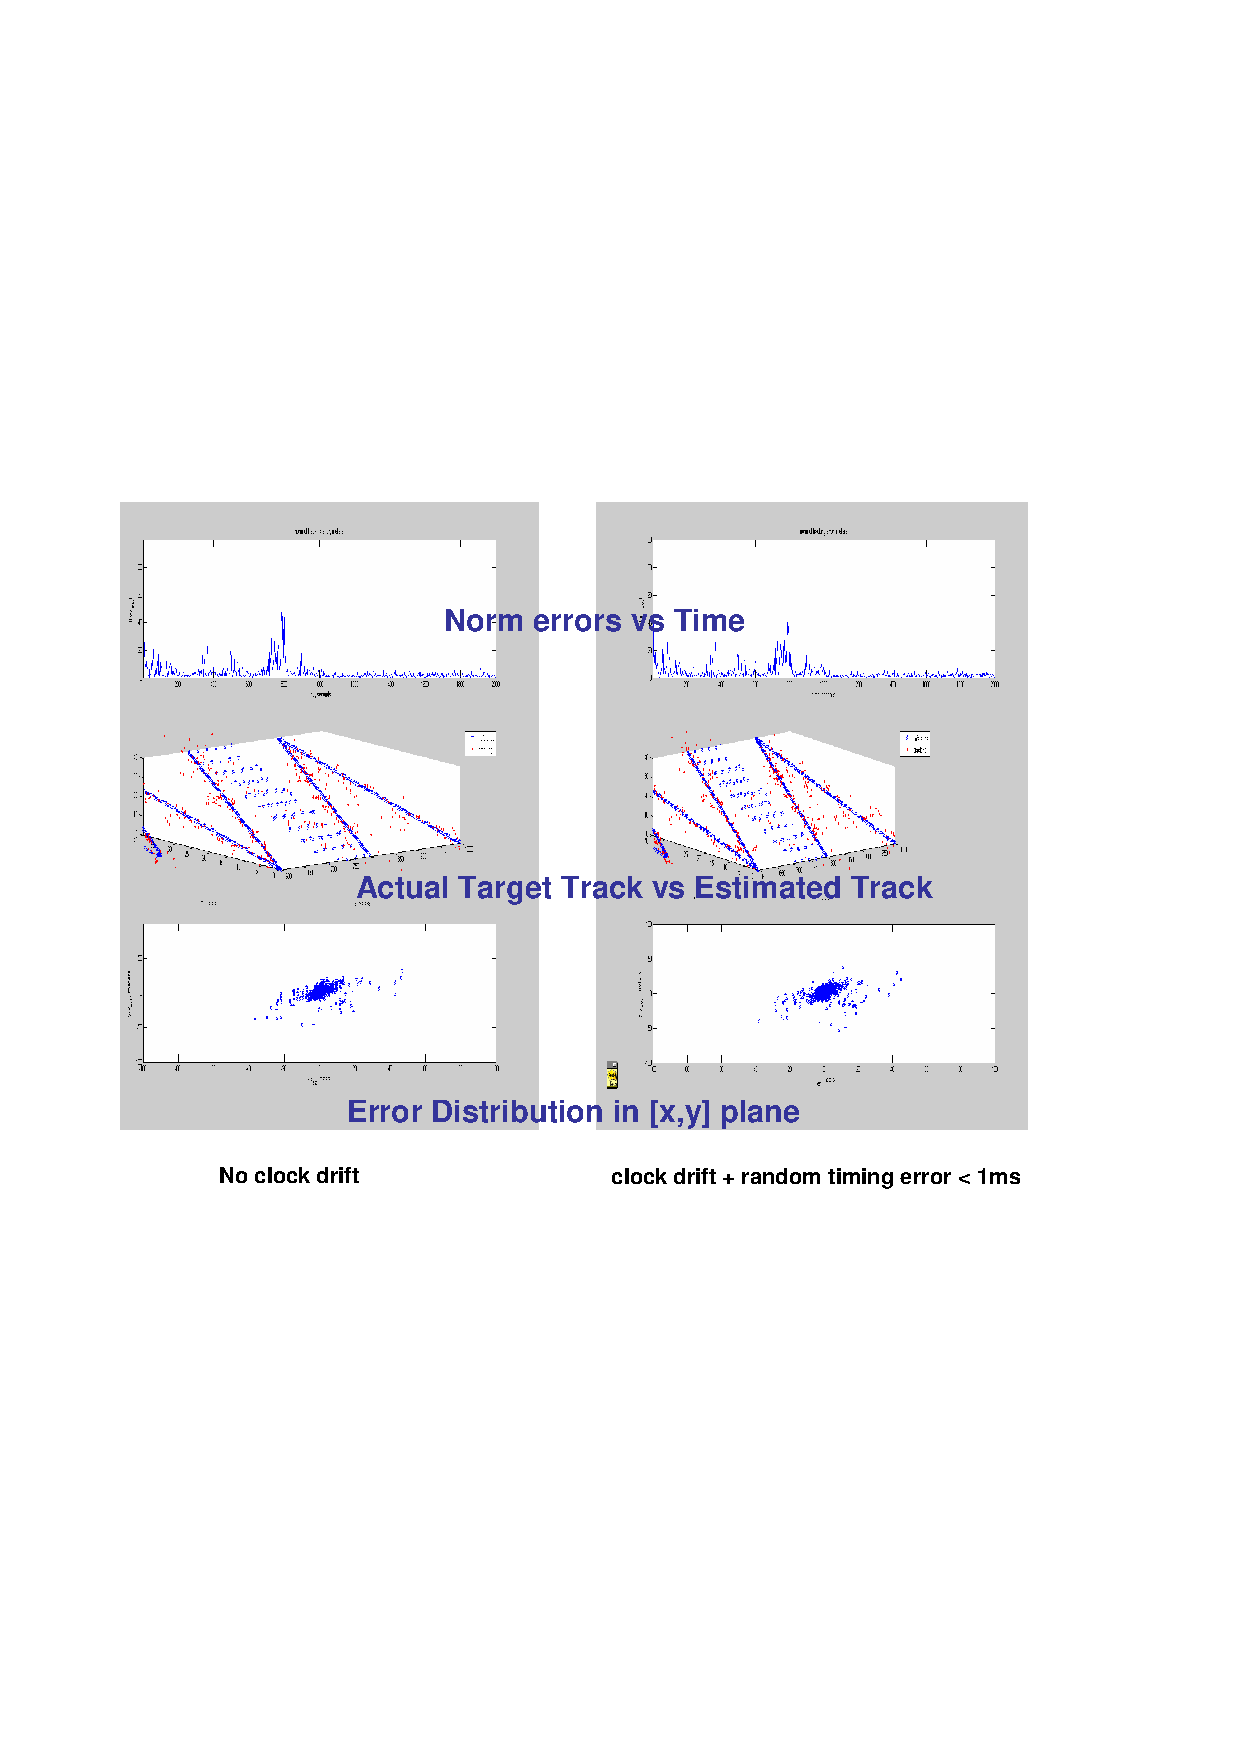
\includegraphics[height=0.45\textheight,width=0.45\textwidth,bbllx=38,bblly=254,bburx=510,bbury=605]{figures/estimationlow}
    \caption{Target Tracking in a low mobility with timing errors. 10 sensors are randomly placed in 50x50 $m^2$ field. Each sensor reports the sample to the target every 5 seconds. The target moves with speed less than 10m/s}
        \label{fig:estimation_low}
    \end{center}
\end{figure}

\begin{figure}
    \begin{center}

    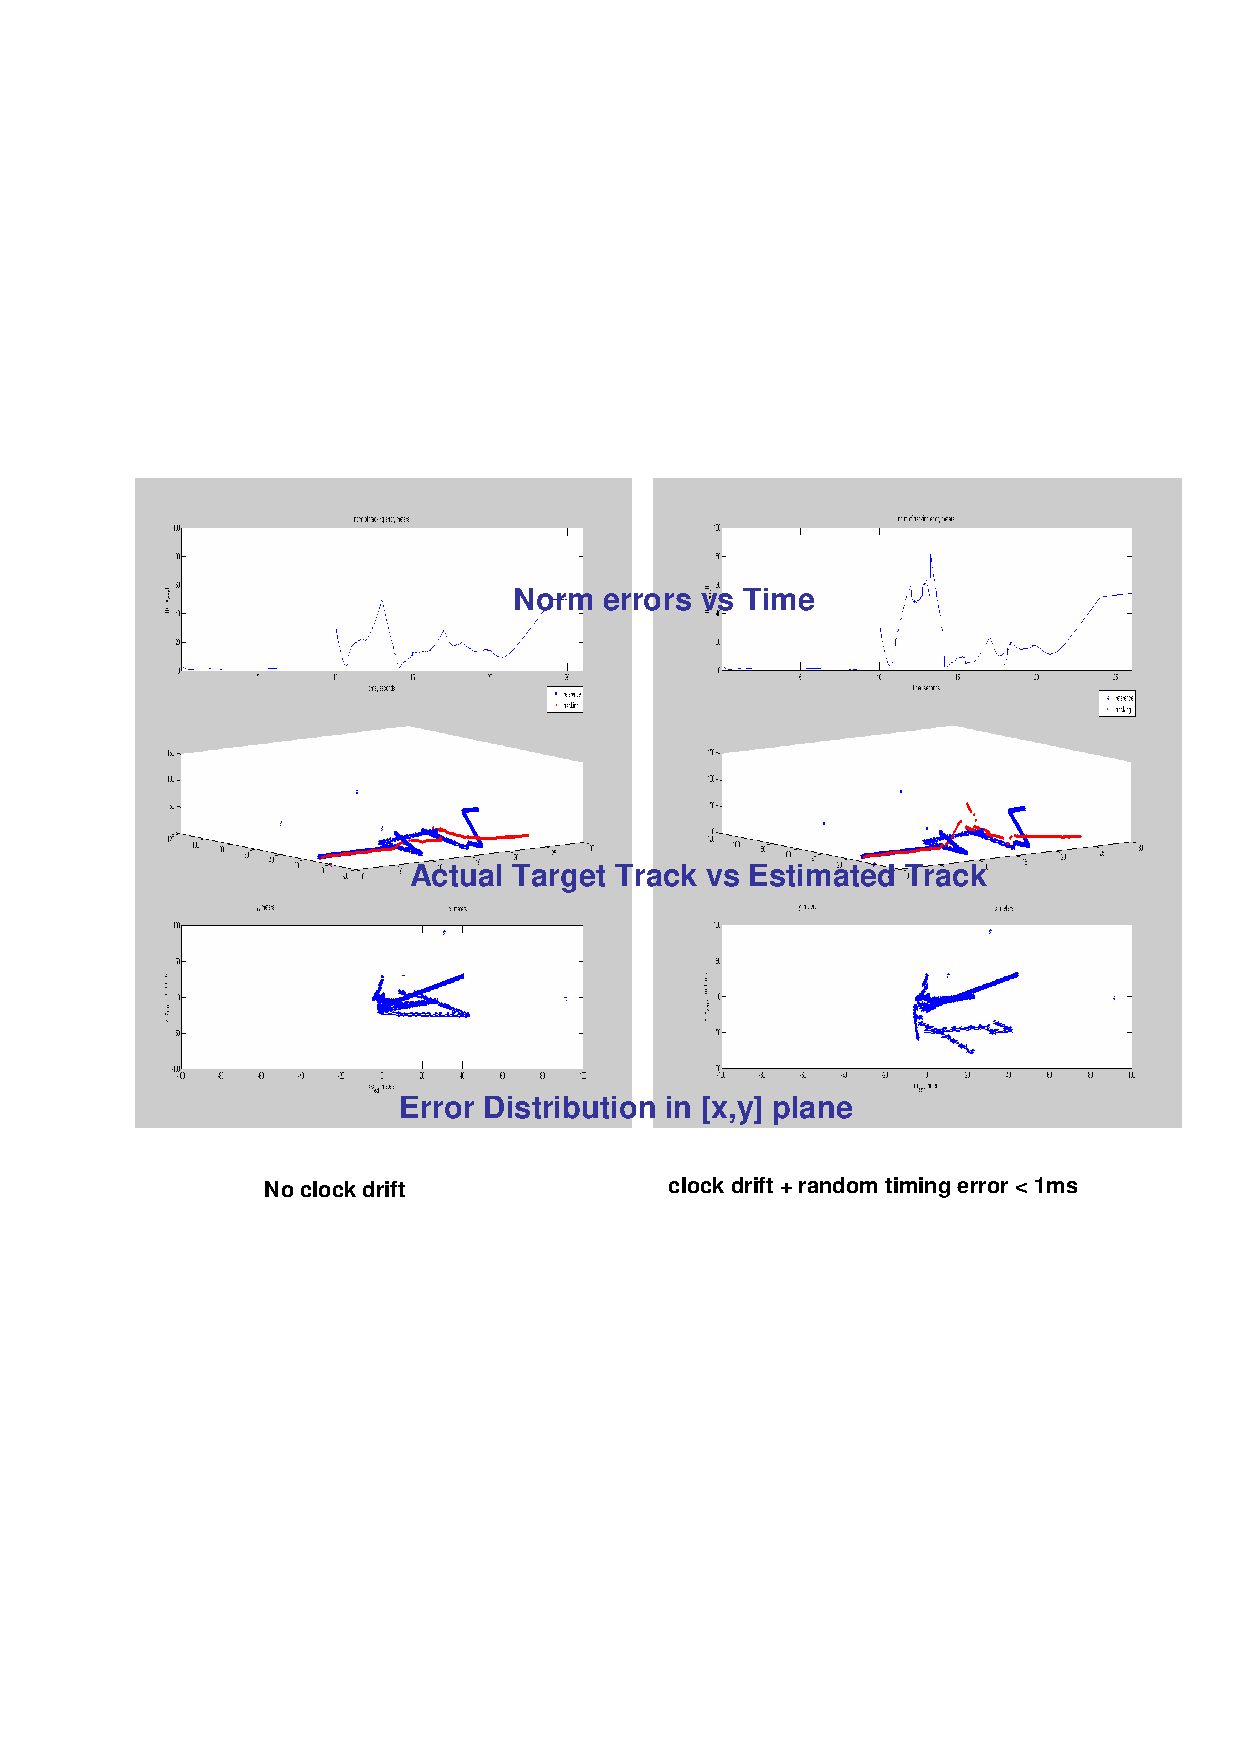
\includegraphics[height=0.45\textheight,width=0.45\textwidth,bbllx=51,bblly=262,bburx=588,bbury=615]{figures/estimationhigh}
    \caption{Target Tracking in a high mobility with timing errors. 10 sensors are randomly placed in 50x50 $m^2$ field. Each sensor reports the sample to the target every 5 seconds. The target moves with speed of 10 $\sim$ 20 m/s. }
        \label{fig:estimation_high}
    \end{center}
\end{figure}

The figures \ref{fig:estimation_low} and \ref{fig:estimation_high}
demonstrate the performance of target tracking using the proposed
filtering algorithm with or without timing errors. Each figure has
three sub-figures. First, it shows the normalized error
$\sqrt{(x'-x_t)^2+(y'-y_t)^2}$ (where $x'$ is the estimated x
location of the target, $x_t$ is the actual location x of the
target) with time. The second graph shows the actual target's
position in blue solid line and the estimated positions in (x,y)
plane in red dotted line. The last diagram shows
([$x'-x_t$,$y'-y_t$]). The results indicate that the filtering is
robust with timing errors less than 1ms. Generally, the
synchronization error through networked time synchronization
mechanisms can achieve less than a few milliseconds error. With high
mobility where target moves faster, the performance degradation with
timing error becomes noticeable. Yet, our scheme is much more robust
to timing errors compared to Least Squares mechanisms shown in
Section \ref{sec:least_square}.

\subsection{Motivation}
The motivation for the above nonlinear hybrid filter was to obtain a filter with globally stable performance (rather than the local stability obtained for an extended Kalman filter), robustness to synchronization errors, inexpensive distributable computation (unlike, for example a particle filter), and the ability to handle uncertainty in sensor location directly. Robustness is accomplished through using a filter with a minimum number of parameters--all of which have a physical significance and do not have to be chosen for specific circumstances of installation of the sensor network. through study of the filter's structure, we see that it is instantaneously unobservable, indeed, the observability matrix for the pair $\left(\mathbf{C}\left(\mathbf{x}(k)\right),\mathbf{A}\right)$ is
\begin{eqnarray}
    \mathbb{O}&=&\left(\begin{array}{c}\mathbf{C}\left(\mathbf{x}(k)\right)\\
    \mathbf{C}\left(\mathbf{x}(k)\right)\mathbf{A}\\
    \mathbf{C}\left(\mathbf{x}(k)\right)\mathbf{A}^2\\
    \mathbf{C}\left(\mathbf{x}(k)\right)\mathbf{A}^3\\
    \mathbf{C}\left(\mathbf{x}(k)\right)\mathbf{A}^4\\
    \mathbf{C}\left(\mathbf{x}(k)\right)\mathbf{A}^5\\
    \end{array}\right)\label{eqn:obsvmatrix}\\
    &=&\begin{pmatrix}
         -m_i & 0 & 0 & 1 & 0 & 0 \\
         0 & -m_i & 0 & 0 & 1 & 0 \\
         0 & 0 & -m_i & 0 & 0 & 1 \\
         0 & 0 & 0 & 0 & 0 & 0 \\
         0 & 0 & 0 & 0 & 0 & 0 \\
         0 & 0 & 0 & 0 & 0 & 0 \\
       \end{pmatrix}
    \label{eqn:obsveig},
\end{eqnarray}
with three non-zero eigenvalues $m_i^2+1$. The intuition for the working of this filter comes from Monte-Carlo methods for thresholding extreme phenomena, where there is short term divergence and long term convergence. We can be reasonably sure of being able to prove the convergence of this filter given that it's tracking error converges to zero in simulations over a wide range of sensor placement, number and tracking object speed. The tools envisioned for this are direct analysis of the sort that is performed for Kalman filters~\cite{SOLO,BOUGEROL}, Barrier certificates to show reliable performance~\cite{PRAJ,GLA}, or stochastic hybrid system tools.

\subsection{Sensitivity to Synchronization Error of Batch Least Squares over the Network}\label{sec:least_square}
This sensitivity analysis applies to least squares or any equivalent
recursive method that attains the least squares solution. We perform
the analysis for a constant velocity model of the tracked object
simply for the purpose of illustration. Suppose that the cartesian
coordinates of a moving object are given the equations
\begin{eqnarray}
x(k)&=&x_0+v_xkT\label{eqn:xconstvel}\\
y(k)&=&y_0+v_ykT\label{eqn:yconstvel},
\end{eqnarray}
then we can construct an array of sequential measurements for the least squares estimation of object position and velocity, with the object of extracting $x_0, v_x, y_0$ and $v_y$. It would have the following form:
\begin{eqnarray}
\mathbb{A}\mathbf{X}&=&\mathbb{B}\label{eqn:batchls1}\\
\mathbb{A}&=&\begin{pmatrix}
               1 & kT & -m_{k,j} &-m_{k,j}kT  \\
               1 & (k+p_1)T & -m_{k+p_1,l} & -m_{k,j}(k+p_1)T \\
               \vdots & \vdots & \vdots & \vdots \\
               1 & (k+p_n)T & -m_{k+p_n,n} & -m_{k+p_n,n}(k+p_n)T \\
             \end{pmatrix}\nonumber\\
\mathbb{B}&=&\begin{pmatrix}
               y_j-m_{k,j}x_j \\
               y_j-m_{k,j}x_j \\
               \vdots \\
               y_n-m_{k+p_n,j}x_n \\
             \end{pmatrix}\nonumber\\
\mathbf{X}&=&\begin{pmatrix}
               y_0 & v_y & x_0 & v_x \\
             \end{pmatrix}^T\nonumber,
\end{eqnarray}
where $T$ is the sample period, $j...n$ are sensor labels, $(x_j,y_j)$ is a sensor position on the plane, $m_{k,j}$ is the slope measurement from sensor $j$ at time $kT$, $k$ going from $k...k+p_n$. From the structure of this least squares problem, if we assume that there are no errors in sensor locations, the synchronization error comes additively into the matrix $\mathbb{A}$ as
\begin{eqnarray}
\mathbb{\delta A}&=&\begin{pmatrix}
               0 & a_0 & 0 &-m_{k,j}a_0 \\
               0 & a_1 & 0 & -m_{k,j}a_1 \\
               \vdots & \vdots & \vdots & \vdots \\
               0 & a_n & 0 & -m_{k+p_n,n}a_n \\
             \end{pmatrix}\label{eqn:ALSError}\\
&=&\begin{pmatrix}
               a_0 \\
               a_1 \\
               \vdots \\
               a_n \\
             \end{pmatrix}^T\begin{pmatrix}
               0 & 1 & 0 &-m_{k,j} \\
               0 & 1 & 0 & -m_{k,j} \\
               \vdots & \vdots & \vdots & \vdots \\
               0 & 1 & 0 & -m_{k+p_n,n} \\
             \end{pmatrix}\label{eqn:ALSError1}\\
&=&\begin{pmatrix}
               a_0 &
               a_1 &
               \hdots &
               a_n
             \end{pmatrix}\delta\mathbb{A'}
\end{eqnarray}
where $a_1,\ldots,a_n$ are the timing errors for the different sensors. For a least squares problem, the first order error in estimation of the unknown given the uncertainty in the regression matrix $\mathbb{A}$ is available from standard references~\cite{BJORK}:
\begin{equation}
\delta \mathbf{X}=\mathbb{A}^\dag\left(\delta \mathbb{B}-\delta\mathbb{A}\mathbf{X}\right)+\left(\mathbb{A}^T\mathbb{A}\right)^{-1}\delta\mathbb{A}^T\mathbf{r},
\end{equation}
where $\mathbf{r}=\mathbb{B}-\mathbb{A}\mathbf{X}$, and $\mathbb{A}^\dag=\left(\mathbb{A}^T\mathbb{A}\right)^{-1}\mathbb{A}^T$ is the More-Penrose inverse of $\mathbb{A}$. If we assume a mean synchronization error of $\bar{a}$ for all of the sensors, we have an estimation error that is directly proportional to it, in the form:
\begin{equation}
\delta \mathbf{X}=-\bar{a}\left(\mathbb{A}^\dag\left(\delta\mathbb{A'}\mathbf{X}\right)-\left(\mathbb{A}^T\mathbb{A}\right)^{-1}\delta\mathbb{A'}^T\mathbf{r}\right),
\end{equation}
 showing that the expected estimation error (assuming that the residual $\mathbf{r}$ is zero mean) is proportional to the product of the synchronization error and the estimate $\mathbf{X}$. Thus, faster object motion or more distant objects will increase the estimation error induced by synchronization error.
